%% Version 4.3.2, 25 August 2014
%
% To-Do
% compare 24-36 hr averages to longterm averages to estimate uncertainty from short % LADCP % stations?
%
%
%
%%%%%%%%%%%%%%%%%%%%%%%%%%%%%%%%%%%%%%%%%%%%%%%%%%%%%%%%%%%%%%%%%%%%%%
% Template.tex --  LaTeX-based template for submissions to the 
% American Meteorological Society
%
% Template developed by Amy Hendrickson, 2013, TeXnology Inc., 
% amyh@texnology.com, http://www.texnology.com
% following earlier work by Brian Papa, American Meteorological Society
%
% Email questions to latex@ametsoc.org.
%
%%%%%%%%%%%%%%%%%%%%%%%%%%%%%%%%%%%%%%%%%%%%%%%%%%%%%%%%%%%%%%%%%%%%%
% PREAMBLE
%%%%%%%%%%%%%%%%%%%%%%%%%%%%%%%%%%%%%%%%%%%%%%%%%%%%%%%%%%%%%%%%%%%%%

%% Start with one of the following:
% DOUBLE-SPACED VERSION FOR SUBMISSION TO THE AMS
%\documentclass{ametsoc}

% TWO-COLUMN JOURNAL PAGE LAYOUT---FOR AUTHOR USE ONLY
\documentclass[twocol]{ametsoc}

%%%%%%%%%%%%%%%%%%%%%%%%%%%%%%%%
%%% To be entered only if twocol option is used

\journal{jtech}

%  Please choose a journal abbreviation to use above from the following list:
% 
%   jamc     (Journal of Applied Meteorology and Climatology)
%   jtech     (Journal of Atmospheric and Oceanic Technology)
%   jhm      (Journal of Hydrometeorology)
%   jpo     (Journal of Physical Oceanography)
%   jas      (Journal of Atmospheric Sciences)	
%   jcli      (Journal of Climate)
%   mwr      (Monthly Weather Review)
%   wcas      (Weather, Climate, and Society)
%   waf       (Weather and Forecasting)
%   bams (Bulletin of the American Meteorological Society)
%   ei    (Earth Interactions)

%%%%%%%%%%%%%%%%%%%%%%%%%%%%%%%%
%Citations should be of the form ``author year''  not ``author, year''
\bibpunct{(}{)}{;}{a}{}{,}

%%%%%%%%%%%%%%%%%%%%%%%%%%%%%%%%

%%% To be entered by author:

%% May use \\ to break lines in title:

\title{A Note on Biases in Turbulent Dissipation Rate Estimated via Thorpe Scales from Profiling Instruments}

%%% Enter authors' names, as you see in this example:
%%% Use \correspondingauthor{} and \thanks{Current Affiliation:...}
%%% immediately following the appropriate author.
%%%
%%% Note that the \correspondingauthor{} command is NECESSARY.
%%% The \thanks{} commands are OPTIONAL.

    %\authors{Author One\correspondingauthor{Author One, 
    % American Meteorological Society, 
    % 45 Beacon St., Boston, MA 02108.}
% and Author Two\thanks{Current affiliation: American Meteorological Society, 
    % 45 Beacon St., Boston, MA 02108.}}

\authors{Andy Pickering\correspondingauthor{Oregon State Unversity, Corvallis OR, USA.}}

%% Follow this form:
    % \affiliation{American Meteorological Society, 
    % Boston, Massachusetts.}

\affiliation{Oregon State Unversity, Corvallis OR USA}

%% Follow this form:
    %\email{latex@ametsoc.org}

\email{andypicke@gmail.com}

%% If appropriate, add additional authors, different affiliations:
    \extraauthor{Jonathan Nash}
    \extraaffil{Oregon State University, Corvallis, OR, USA}

%\extraauthor{}
%\extraaffil{}

%% May repeat for a additional authors/affiliations:

\extraauthor{Matthew Alford}
\extraaffil{Scripps Institute of Oceanography}

%%%%%%%%%%%%%%%%%%%%%%%%%%%%%%%%%%%%%%%%%%%%%%%%%%%%%%%%%%%%%%%%%%%%%
% ABSTRACT
%
% Enter your abstract here
% Abstracts should not exceed 250 words in length!
%
% For BAMS authors only: If your article requires a Capsule Summary, please place the capsule text at the end of your abstract
% and identify it as the capsule. Example: This is the end of the abstract. (Capsule Summary) This is the capsule summary. 

\abstract{Data from fast-sampling thermistor moorings are used to diagnose and quanitfy the errors in turbulent dissipation rate of kinetic energy $\epsilon$ ($\mathrm{Wkg^{-1}}$) computed from Thorpe scales when measured by a profiling instrument. Two main sources of errors are identified and quantified. First, the profiler under-samples the density field, resulting in zero bias but a nonzero uncertainty that is inversely proportional to sampling speed. Second, each �profile� is not actually measured instantaneously as normally assumed, but rather sampled over a finite time period during which the background density field may change. This can introduce false overturns in a stable profile, as well as measured overturns that are larger or smaller than the true size. We quantify these effects are by resampling moored temperature measurements to simulate sampling by a profiling instrument at various speeds. The error in $\epsilon$ is proportional to the (true) size of the overturn. The results are applicable to commonly used profiling instruments such as the McLane moored profiler and the shipboard CTD.}

\begin{document}

%% Necessary!
\maketitle


%%%%%%%%%%%%%%%%%%%%%%%%%%%%%%%%%%%%%%%%%%%%%%%%%%%%%%%%%%%%%%%%%%%%%
% MAIN BODY OF PAPER
%%%%%%%%%%%%%%%%%%%%%%%%%%%%%%%%%%%%%%%%%%%%%%%%%%%%%%%%%%%%%%%%%%%%%
%

%% In all cases, if there is only one entry of this type within
%% the higher level heading, use the star form: 
%%
% \section{Section title}
% \subsection*{subsection}
% text...
% \section{Section title}

%vs

% \section{Section title}
% \subsection{subsection one}
% text...
% \subsection{subsection two}
% \section{Section title}

%%%
% \section{First primary heading}

% \subsection{First secondary heading}

% \subsubsection{First tertiary heading}

% \paragraph{First quaternary heading}


\section{Introduction}

Turbulence is an important oceanographic variable, responsible for vertical mixing of nutrients, pollutants, heat, and salt. Turbulent mixing also helps maintain the ocean�s meridional overturning circulation by mixing dense abyssal water with lighter water above \citep{munk66,munkwunsch98}. Climate models are sensitive to the location and magnitude of turbulent mixing \citep{jayne09,meletetal13}, but generally do not resolve the smalls scales at which it occurs, so they must be parameterized.

However, direct measurement of turbulence is difficult. The gold standard is direct measurement by specialized thermistors or shear probes that resolve the small (mm) scales where turbulent dissipation takes place. These instruments are expensive and require specialized personnel to maintain, operate, and analyze. This technology has improved greatly and there are now some commercially available turbulence profilers, but they remain expensive and require more skill and care to operate. Because of these factors, the number and spatial coverage of turbulence measurements over the oceans remains sparse \citep{waterhouseetal14}.

In contrast, CTD profiles of temperature and salinity are relatively easy and cheap to acquire, and far more data is available. For these reasons, estimating turbulence from CTD profiles with Thorpe Scale analysis has become a common technique. Though not a direct measurement of turbulence, estimates of turbulent dissipation rates from overturns have been shown to compare relatively well with direct measurements \citep{dillon82}. Several studies have investigated the errors in this method resulting from instrument noise, sampling rate, and water-mass intrusions \citep{ferronetal98,galbraithkelley96}. There are also remaining questions about the validity of assumptions going into the calculation, such as whether $L_T/L_o$ is constant, and the assumed mixing efficiency. We do not address these issues in this paper; our focus is only on the error induced by samping from a profiling instrument.

In applying the Thorpe scale method, there is an implicit assumption that profiles were made instantaneously, or that the true profile of temperature or density did not change during the time it took for a profile. The validity of this assumption and its effect on the estimated turbulence has not been investigated (though it was pointed out by \cite{thorpe77}), and is the subject of this paper. During the time taken to complete a profile, the density structure and turbulence may change or be advected by the lower-frequency background flow. Vertical advection during a profile may decrease or increase the apparent overturn size measured by the instrument, and in some cases can introduce apparent overturns in a profile that is actually stable. %To study these effects, we simulate sampling by a profiling instrument. 


%~~~~~~~~~~~~~~~
\section{Data}

The data used in this study come from an array of thermistor moorings deployed in Luzon Strait during the Internal Waves in Straits Experiment (IWISE). The moorings were deployed in a zonal line on the eastern slope of the western ridge, where previous measurements and models indicated strong overturns and turbulent dissipation associated with breaking lee waves formed by tidal flow over the ridge \citep{alfordetal11b,buijsmanetal12}. Instruments included SBE-56's, SBE-37's and RBR-1060's, all sampling at 1 second intervals. The average vertical spacing between instruments was about 50m. For this study, all measurements were corrected for mooring blowdown using pressure measured by the SBE-37 Microcats, and then interpolated onto a depth-time grid grid with vertical spacing of 10m and temporal interval of 2 minutes.

%~~~~~~~~~~~~~~~
\section{Methods}

\subsection{Thorpe Scale Analysis}
Overturns are computed from potential temperature profiles using now well-established methods. \cite{thorpe77} proposed that the size of overturns in potential density profiles could be related to the size of turbulent eddies and the turbulent dissipation rate. Profiles of potential  temperature (in this data there is a tight temperature-density relation) are sorted to form stable profiles. The distance each parcel of water must be moved vertically is defined as the Thorpe displacement $L$. The Thorpe scale $L_{T}$ is defined as the rms Thorpe displacement over each overturning region. The Thorpe scale is assumed to be proportional to the Ozmidov scale $L_O$ \citep{ozmidov65}, the maximum overturning length scale in a stratified fluid; this relationship has been found experimentally to be $L_O=0.8L_{T}$ \citep{dillon82}. Using the relationship between $L_O$ and $\epsilon$ $L_O=\epsilon^{1/2}N^{-3/2}$, turbulent dissipation rate is computed as $\epsilon=0.64L_{T}^{2}N^3$, where $N$ is the mean buoyancy frequency over each overturning region, computed from the sorted profile. 

Spurious overturns are identified and rejected using several standard tests, including statistical run-length tests \citep{galbraithkelley96} and instrument noise levels \citep{ferronetal98}. However in this case, the minimum resolvable overturn is set by the coarse vertical instrument spacing (about 50 m). At typical open ocean levels of turbulence, this sampling would be too coarse to resolve most of the overturns. However, it is sufficient to resolve the very strong turbulence at this location, which is dominated by large overturns (greater than 50m). 

We use data from T-chains 3 and 4 in this study. Turbulence at moorings 1 and 2 was dominated by smaller overturns and not as well-resolved by the thermistor moorings. We will examine the effects on two commonly-used quanitites of $\epsilon$: the depth-integrated dissipation rate, and the time-average profile.
 
%~~
\subsection{Resampling}

The full data are resampled to simulate measurement by a profiling instrument traveling up and down at a constant vertical speed at a fixed spatial location (i.e. mooring or ship CTD, not gliders). Two commonly-used instruments are McLane Moored Profilers (MPs) and shipboard CTDs. The data is then resampled by interpolating the full T-chain data onto the depth-time path of a profiling instrument for a given speed. Each up or down segment of the path (Figure \ref{T3ExamSamp}) results in one �profile� at the time of the midpoint of the segment. The same Thorpe scale analysis is then applied to these resampled profiles. The resampling is done for an ensemble of sampling paths with the start time shifted by 2 mins, in order to average over all possible phases between sampling and the flow. For this analysis, we use data from yearday 165 to 185, a period encompassing an entire spring cycle during which all instruments were functioning. The Matlab code used to resample data along simulated profiles is available at \url{https://github.com/andypicke/SimProfiler}.

%~~
\section{Results}


%~~~
\subsection{Effect of under-sampling}

We first examine the error associated only with under-sampling (in time) of the true temperature field. The true profiles are sampled at time intervals corresponding to the time it would take for one profile at a given sampling speed, and the average dissipation rate is computed. This process is repeated for an ensemble of different start times for each profiling speed (Figure \ref{T3undersamp}). The mean of each ensemble is approximately equal to the true mean (i.e. there is no bias), but the standard deviation is non-zero and inversely proportional to the profiling speed. 

%~~~
\subsection{Effect of non-instantaneous profiles}

Next we examine the effect of non-instantaneous profiles sampled by a profiling instrument at 4 different speeds. The $0.25\mathrm{ms^{-1}}$ case simulates sampling by a McLane moored profiler (MP). Note that the MP can be slowed or stopped from crawling by strong vertical velocities, meaning that the uncertainties presented here are likely a lower limit. The ensemble mean profiles have a positive bias that is inversely proportional to the profiling speed (Figure \ref{T3profsDiffSpeeds2X2}). The ensemble mean profile is biased by approximately a factor of 2 for $w=0.25\mathrm{ms^{-1}}$. Time-series of the depth integrated dissipation averaged over one day (Figure \ref{T3_TS_DiffSpeeds2X2}) exhibit similar results. 

%~~~
\subsubsection{Histograms}

Figure \ref{hists} shows histograms of overturn size for the true T-chain data as well as the resampled data for $w=0.15$. Distributions of overturn size and Thorpe scale are similar, but the resampled data contains larger values than the true value. Histograms of $N^2$ are both approximately lognormal, but the resampled data are shifted to larger values. Epsilon is similar, with resample data exhibiting a similar distribution shifted to larger values. Larger Thorpe scales and $N^2$ will both lead to larger values of epsilon, with stratification having a larger impact since $\epsilon \propto N^3$.

%~~~
\subsubsection{CTD Scenario}

We also present another scenario designed to simulate continuous CTD sampling (such as 24-36 hour LADCP/CTD stations) since it is such a common measurement. The typical profiling speed for a shipboard CTD is $1\mathrm{ms^{-1}}$, ignoring the short sections of the water column near the top and bottom where it is normally slowed. We also simulate sampling on the downcast only, which is often done since water is contaminated by the CTD package's wake on upcasts. The sampling results in an average bias close to zero (Figure \ref{T3_ctd_profile}), but significant uncertainty for individual profiles. It seems that the profile speed of the CTD is high enough to significantly reduce the errors and bias from non-instantaneous profiles seen at lower speeds, but the under-sampling from using only the downcasts increases the uncertainty.


%~~~~~~~~~~~~~~~~
%\section{Mechanisms}


%~~~
\subsection{Detailed Look at One Turbulent Cycle}

Next we look at one turbulent period in detail to gain a better understanding of what leads to the bias. In Figure \ref{zoomex}, resampled $\epsilon$ is plotted along downward and upward sampling paths. It is clear that the bias is largest when the slope of isopycnals are approximately equal to the slope of the profiling path in depth-time space (or equivalently, the `background' vertical velocity of the fluid is equal to that of the profiler). 


%~~~
\subsection{Why is the Bias Always Positive?}

We imagine an instrument profiling through a density field containing turbulent overturns with the `true' size equal to what would measured by an instantaneous profile at the midpoint of the slower profile. During the time taken to complete a profile, the background field may evolve and overturns may be advected vertically or horizontally (we neglect horizontal advection here). If the advection is in the direction of the profiler, the measured overturn should appear larger than the true size. If advection is in the opposite direction, overturns will be compressed and appear smaller. Assuming the phase between the sampling and any vertical advection is random, the measured overturns will be symmetrically perturbed to smaller and larger values and have the same average size. However because $\epsilon \propto L_{T}^{2}$, the average $\epsilon$ will be larger than the true value, resulting in a positive bias. We can also test this model by examining histograms of the difference between true and resampled overturn sizes (Figure \ref{T3LtDiffHists}), which are approximately normally distributed with a mean near zero. The width (standard deviation) of the distribution decreases with increasing sampling speed, supporting this hypothesis.


%~~~
\subsection{Dependence on overturn size}

The bias appears to scale nearly linearly with the magnitude of the true dissipation rate. This is likely because in general larger overturns are associated with larger vertial velocities. * Do we need this figure too?*


%~~~~~~~~~~~~~~~~~~~~~~
\subsection{Identifying and Correcting Biased Data}

Can we identify errors in epsilon from the sampled data without knowledge of the `true' data? One method would be to identify regions where the background vertical velocity is similar to the profiler speed. However, the slow sampling prohibits accurate estimation of vertical velocity over the timescales we are interested in. Instead, we infer a turbulent velocity $w_t$ velocity scale based on the measured Thorpe scale and stratification, $w_{t}=L_TN$. Data where $w_t$ is larger than a fraction of the profiler speed $w_{samp}$ are marked as biased and discarded. For data at T-chain 3, we found that the criteria $w_t > 0.5 w_{samp}$ eliminated most of the bias in the time-averaged profile of epsilon (Figure \ref{T3_corrProf}).


%~~~~~~~~~~~~~~~~
\section{Discussion}

Due to the expense and difficulty of making direct turbulence measurements, Thorpe scale analyses of CTD or MP profiles are likely to remain an important source of mixing observations  into the foreseeable future. New instruments and techniques such as $\chi$-pods deployed on WOCE CTD measurements (ref?) should increase the number and quality of turbulence measurements, but still require more expense and expertise, and are greatly outnumbered by the available CTD profiles. Thorpe scale analysis is also often the only means of estimating past mixing levels from historical CTD profiles. 

These results provide useful constraints for planning sampling by mooring or shipboard CTD. Obviously faster sampling speeds are preferred, but the profiling speed of a MP or CTD is typically fixed. Reducing the vertical range of the profiler can reduce uncertainty due to undersampling, but will not help the problem of vertical velocities similar to the profiler speed. Preliminary full-depth measurements and local model simulations could help identify specific depths to be studied, allowing measurements to be optimized for estimating turbulence. 

Do the results of this study apply to other locations? The magnitude of the bias will likely vary depending on the nature of flow and turbulence at different locations, but we expect the relationship between bias and profiling speed to be similar at most locations. We also expect the positive bias to hold at most locations, as a result of the two mechanisms discussed in the previous section. However, the results presented here are for a particular location, and may differ at other locations with different flow regimes and turbulent processes. Similar analysis with other highly-resolved timeseries should provide more information on this.


%~~~~~~~~~~~~~~~~~~~~
\section{Conclusions}

We have shown that Thorpe-scale estimates of $\epsilon$ from data measured by profiling instruments can exhibit a positive bias that is inversely proportional to the vertical sampling speed. Under-sampling of the true temperature field results in uncertainty but zero bias. `Profiles' measured over a finite time result in errors and a positive bias. Errors are largest when the background vertical velocity is close to that of the profiler. The results suggest that errors are minimal for CTD sampling at typical speeds of about $1$m/s. At slower sampling speeds more typical of moored profilers, there can be a significant bias in energetic regions with large vertical displacements. The results should be useful in estimating uncertainty in turbulent dissipation rates measured from overturns by profiling instruments, as well as in planning sampling of turbulent overturns.

%Since $\epsilon$ is proportional to $L_{T}^{2}$, this will also result in a higher average

%%%%%%%%%%%%%%%%%%%%%%%%%%%%%%%%%%%%%%%%%%%%%%%%%%%%%%%%%%%%%%%%%%%%%
% ACKNOWLEDGMENTS
%%%%%%%%%%%%%%%%%%%%%%%%%%%%%%%%%%%%%%%%%%%%%%%%%%%%%%%%%%%%%%%%%%%%%
%
\acknowledgments
Funded by ONR. Everyone who helped with mooring deployments and recovery.

%%%%%%%%%%%%%%%%%%%%%%%%%%%%%%%%%%%%%%%%%%%%%%%%%%%%%%%%%%%%%%%%%%%%%
% APPENDIXES
%%%%%%%%%%%%%%%%%%%%%%%%%%%%%%%%%%%%%%%%%%%%%%%%%%%%%%%%%%%%%%%%%%%%%
%
% Use \appendix if there is only one appendix.
%\appendix

% Use \appendix[A], \appendix}[B], if you have multiple appendixes.
%\appendix[A]

%% Appendix title is necessary! For appendix title:
%\appendixtitle{}

%%% Appendix section numbering (note, skip \section and begin with \subsection)
% \subsection{First primary heading}

% \subsubsection{First secondary heading}

% \paragraph{First tertiary heading}

%% Important!
%\appendcaption{<appendix letter and number>}{<caption>} 
%must be used for figures and tables in appendixes, e.g.,
%
%\begin{figure}
%\noindent\includegraphics[width=19pc,angle=0]{figure01.pdf}\\
%\appendcaption{A1}{Caption here.}
%\end{figure}
%
% All appendix figures/tables should be placed in order AFTER the main figures/tables, i.e., tables, appendix tables, figures, appendix figures.
%
%%%%%%%%%%%%%%%%%%%%%%%%%%%%%%%%%%%%%%%%%%%%%%%%%%%%%%%%%%%%%%%%%%%%%
% REFERENCES
%%%%%%%%%%%%%%%%%%%%%%%%%%%%%%%%%%%%%%%%%%%%%%%%%%%%%%%%%%%%%%%%%%%%%
% Make your BibTeX bibliography by using these commands:
 \bibliographystyle{ametsoc2014}
 \bibliography{/Users/Andy/Cruises_Research/wavebib/main.bib}


%%%%%%%%%%%%%%%%%%%%%%%%%%%%%%%%%%%%%%%%%%%%%%%%%%%%%%%%%%%%%%%%%%%%%
% TABLES
%%%%%%%%%%%%%%%%%%%%%%%%%%%%%%%%%%%%%%%%%%%%%%%%%%%%%%%%%%%%%%%%%%%%%
%% Enter tables at the end of the document, before figures.
%%
%
%\begin{table}[t]
%\caption{This is a sample table caption and table layout.  Enter as many tables as
%  necessary at the end of your manuscript. Table from Lorenz (1963).}\label{t1}
%\begin{center}
%\begin{tabular}{ccccrrcrc}
%\hline\hline
%$N$ & $X$ & $Y$ & $Z$\\
%\hline
% 0000 & 0000 & 0010 & 0000 \\
% 0005 & 0004 & 0012 & 0000 \\
% 0010 & 0009 & 0020 & 0000 \\
% 0015 & 0016 & 0036 & 0002 \\
% 0020 & 0030 & 0066 & 0007 \\
% 0025 & 0054 & 0115 & 0024 \\
%\hline
%\end{tabular}
%\end{center}
%\end{table}

\clearpage

%%%%%%%%%%%%%%%%%%%%%%%%%%%%%%%%%%%%%%%%%%%%%%%%%%%%%%%%%%%%%%%%%%%%%
% FIGURES
%%%%%%%%%%%%%%%%%%%%%%%%%%%%%%%%%%%%%%%%%%%%%%%%%%%%%%%%%%%%%%%%%%%%%
%% Enter figures at the end of the document, after tables.
%%
%
%\begin{figure}[t]
%  \noindent\includegraphics[width=19pc,angle=0]{figure01.pdf}\\
%  \caption{Enter the caption for your figure here.  Repeat as
%  necessary for each of your figures. Figure from \protect\cite{Knutti2008}.}\label{f1}
%\end{figure}


%~~~~~~~~~~~
\begin{figure}[t]
  \noindent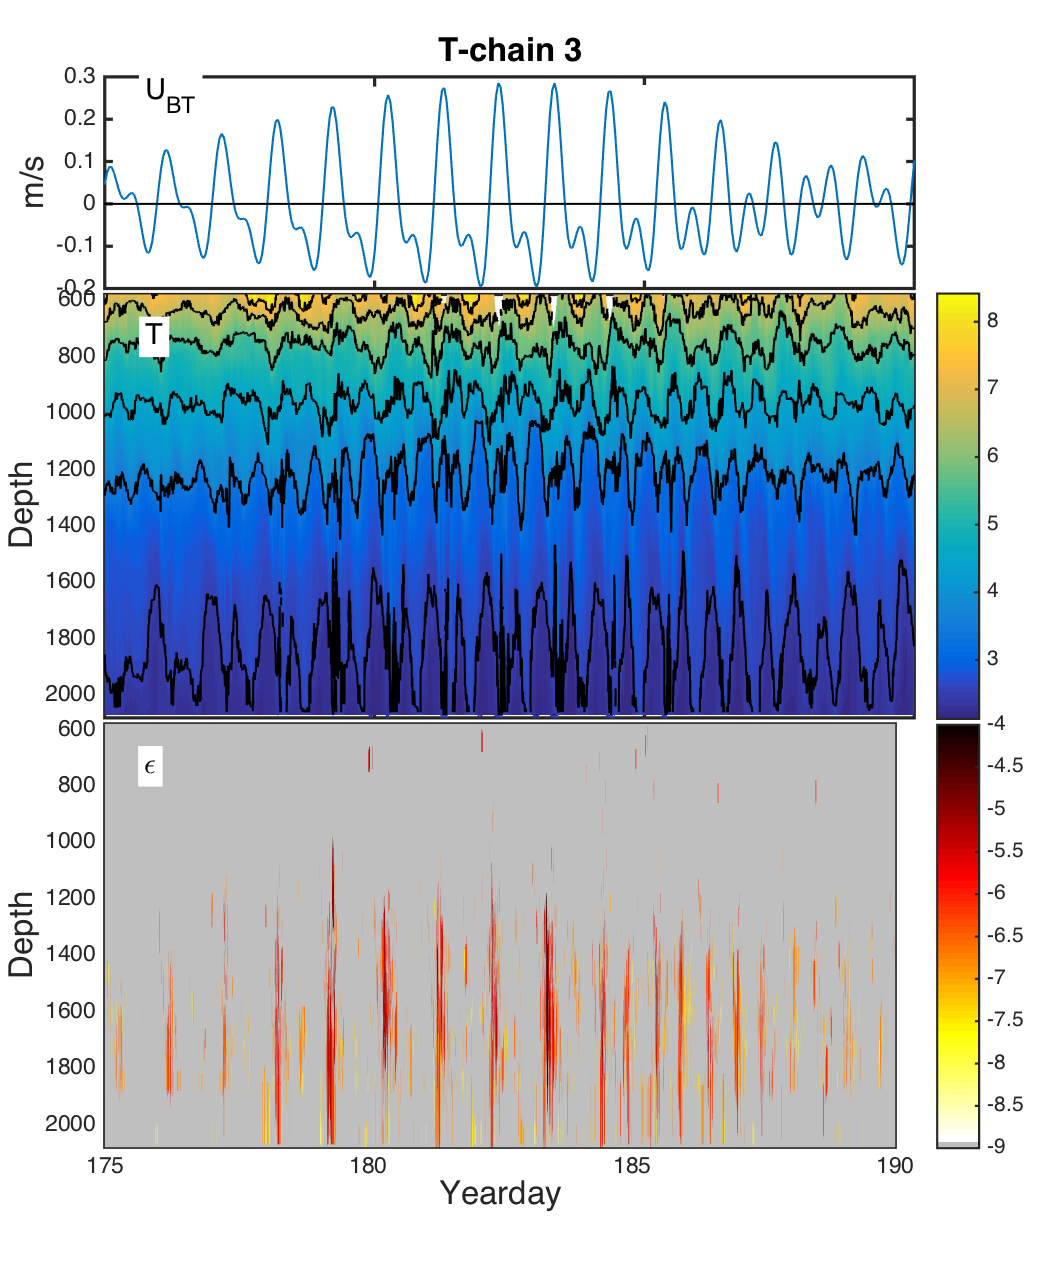
\includegraphics[width=38pc,angle=0]{../NotesOverturnBiases/Tchain3_Overview.png}\\
  \caption{Example data from T-chain 3. (Top) Barotropic tidal velocity from TPXO. (Middle) Temperature. (Bottom) Turbulent dissipaiton rate epsilon. * mark time period of zoom-in Fig \ref{T3ExamSamp}}
  \label{}
\end{figure}


%~~~~~~~~~~~
\clearpage
%PlotShortSectionPaper.m
\begin{figure}[t]
  \noindent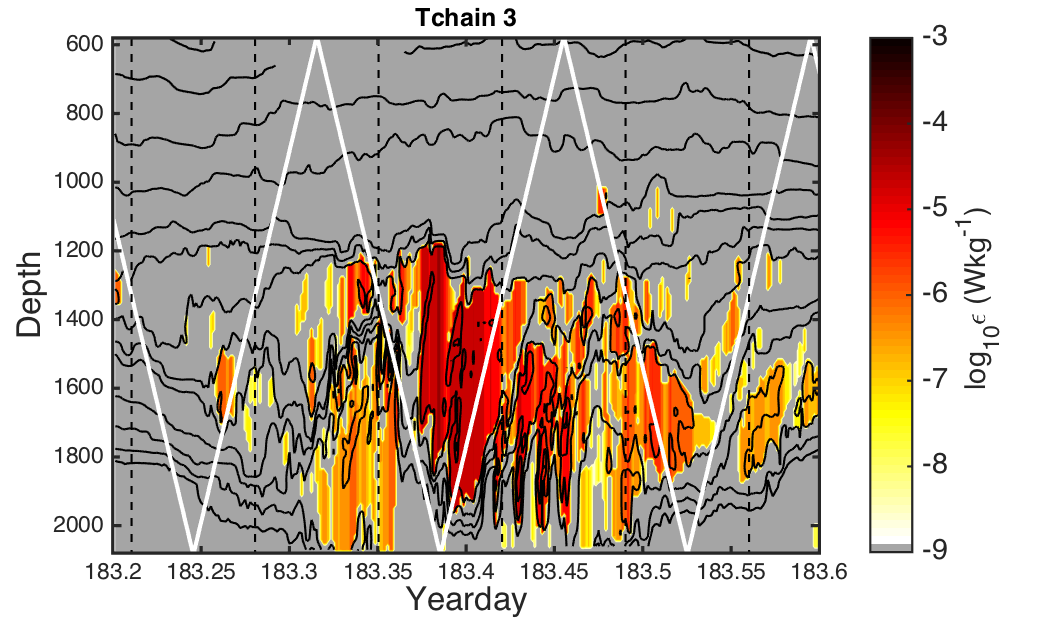
\includegraphics[width=38pc,angle=0]{../NotesOverturnBiases/Tchain3_ExampleSample.png}\\
  \caption{Example data from T-chain 3. Showing epsilon (color) and isotherms (black). White line shows an example sampling path for $w=0.25\mathrm{ms^{-1}}$. Dashed vertical lines indicate midpoint time of profiles.}
  \label{T3ExamSamp}
\end{figure}


%~~~~~~~~~~~
\clearpage
%~~~ under-sampling
\begin{figure}[t]
  \noindent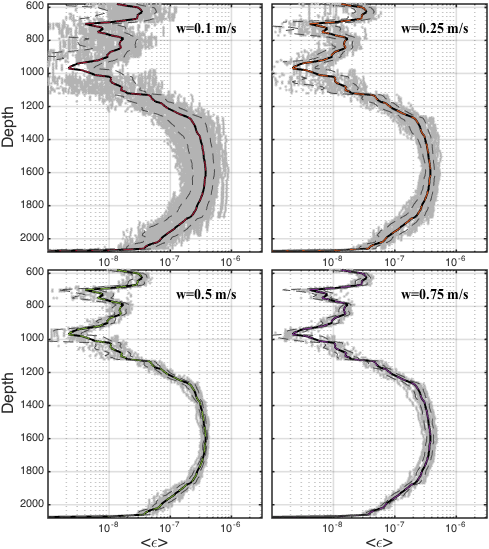
\includegraphics[width=38pc,angle=0]{../NotesOverturnBiases/Tchain3_UnderSamp_4speeds.png}\\
  \caption{Profiles of time-average dissipation rate due to under-sampling only at different speeds. Black is true profile using all data. Gray are profiles for ensemble of simulated under-sampling. Yellow is the ensemble mean, showing that bias is zero. Each panel shows results for a different profiling speed, increasing from left to right and top to bottom. Note that the uncertainty is inversely proportional to sampling speed, but the bias is zero in all cases.}
  \label{T3undersamp}
\end{figure}



%~~~~~~~~~~~
\clearpage
% depth-profiles
\begin{figure}[t]
  \noindent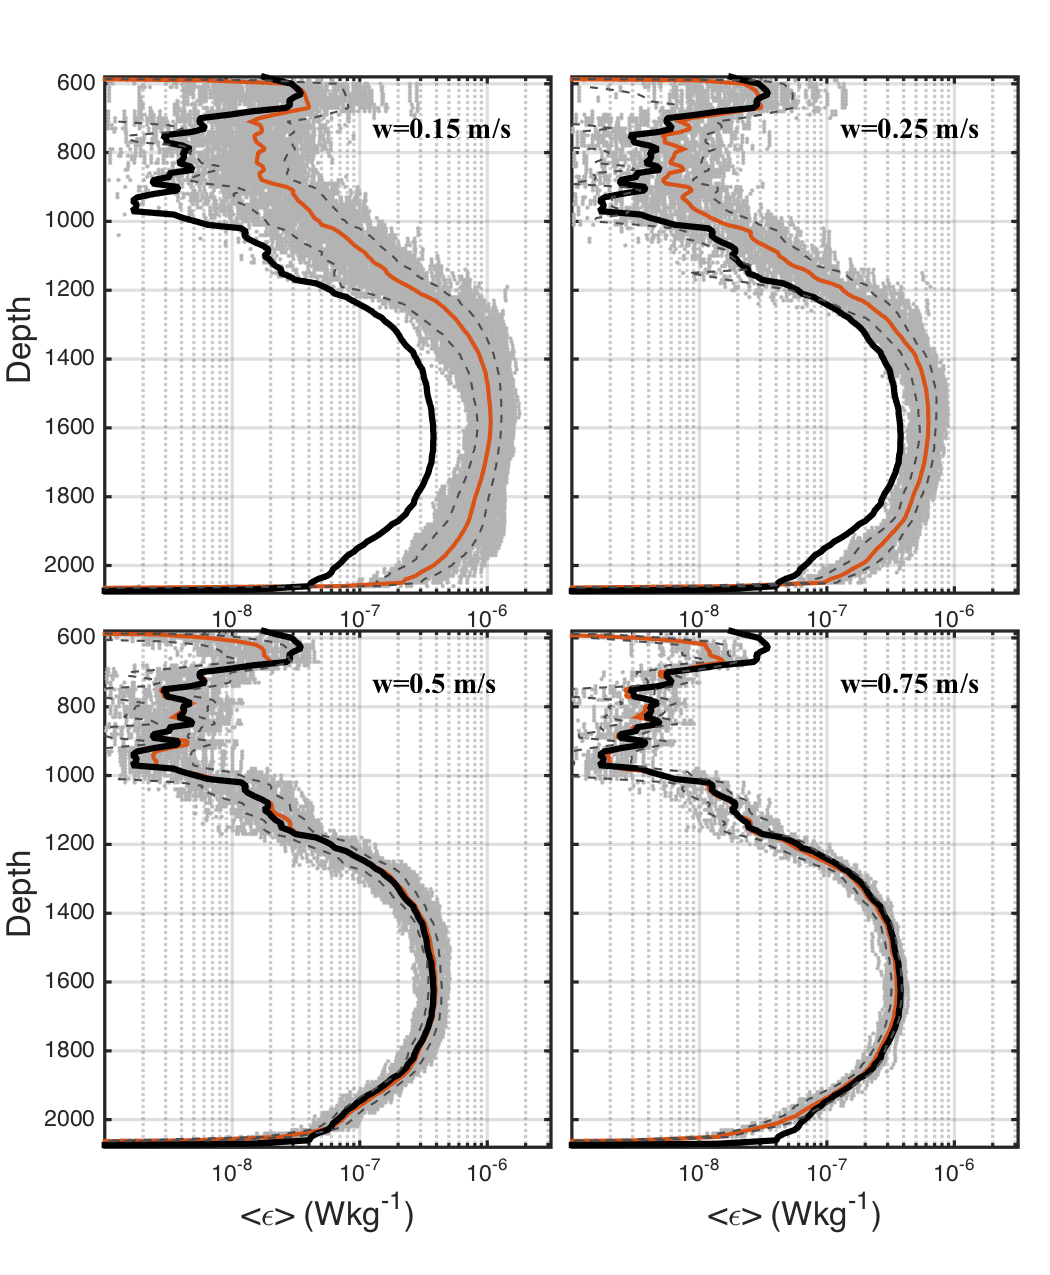
\includegraphics[width=38pc,angle=0]{../NotesOverturnBiases/Tchain3_Resamp_EpsvsDepth_DiffSpeeds_2X2.png}\\
  \caption{Time-mean profiles of dissipation rate at T-chain 3 for different profiling speeds. Black line is true profile using all data. Yellow line is mean of resampled ensemble. Gray is all individual resample profiles. Dashed lines indicate $\pm$ 1 standard deviation.}
  \label{T3profsDiffSpeeds2X2}
\end{figure}


%~~~~~~~~~~~
\clearpage
% time series
\begin{figure}[t]
  \noindent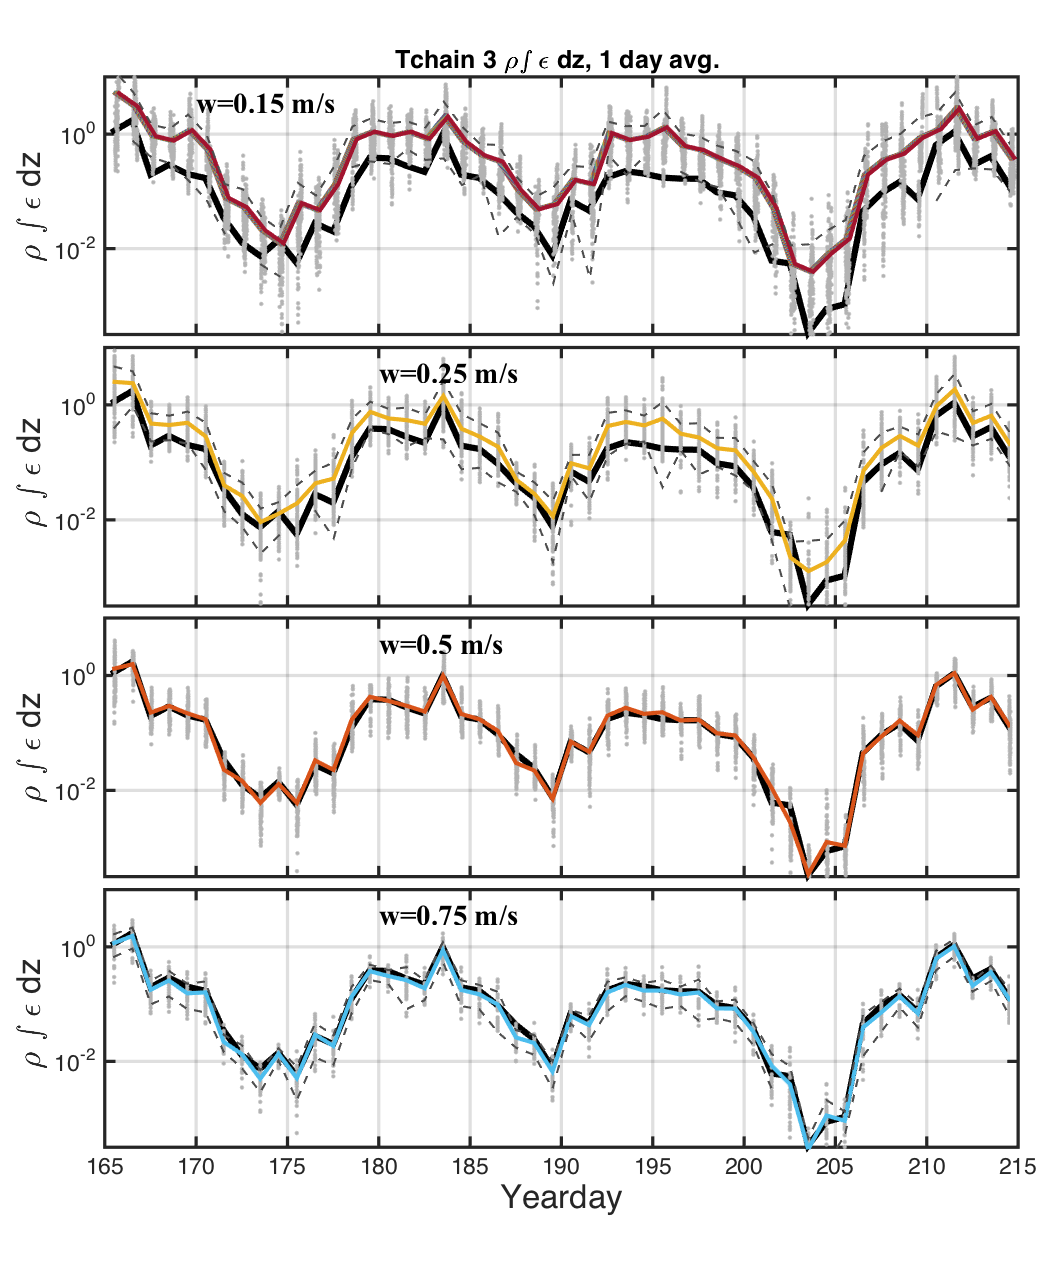
\includegraphics[width=38pc,angle=0]{../NotesOverturnBiases/Tchain3_Resamp_IntEpsvsTime_DiffSpeeds_2X2.png}\\
  \caption{Depth-integrated time series of dissipation rate at T-chain 3 for different profiling speeds. Black line is true profile using all data. Yellow line is mean of resampled ensemble. Gray is all individual resample profiles. Dashed lines indicate $\pm$ 1 standard deviation.}
  \label{T3_TS_DiffSpeeds2X2}
\end{figure}


%~~~~~~~~~~~
\clearpage
\begin{figure}[t]
  \noindent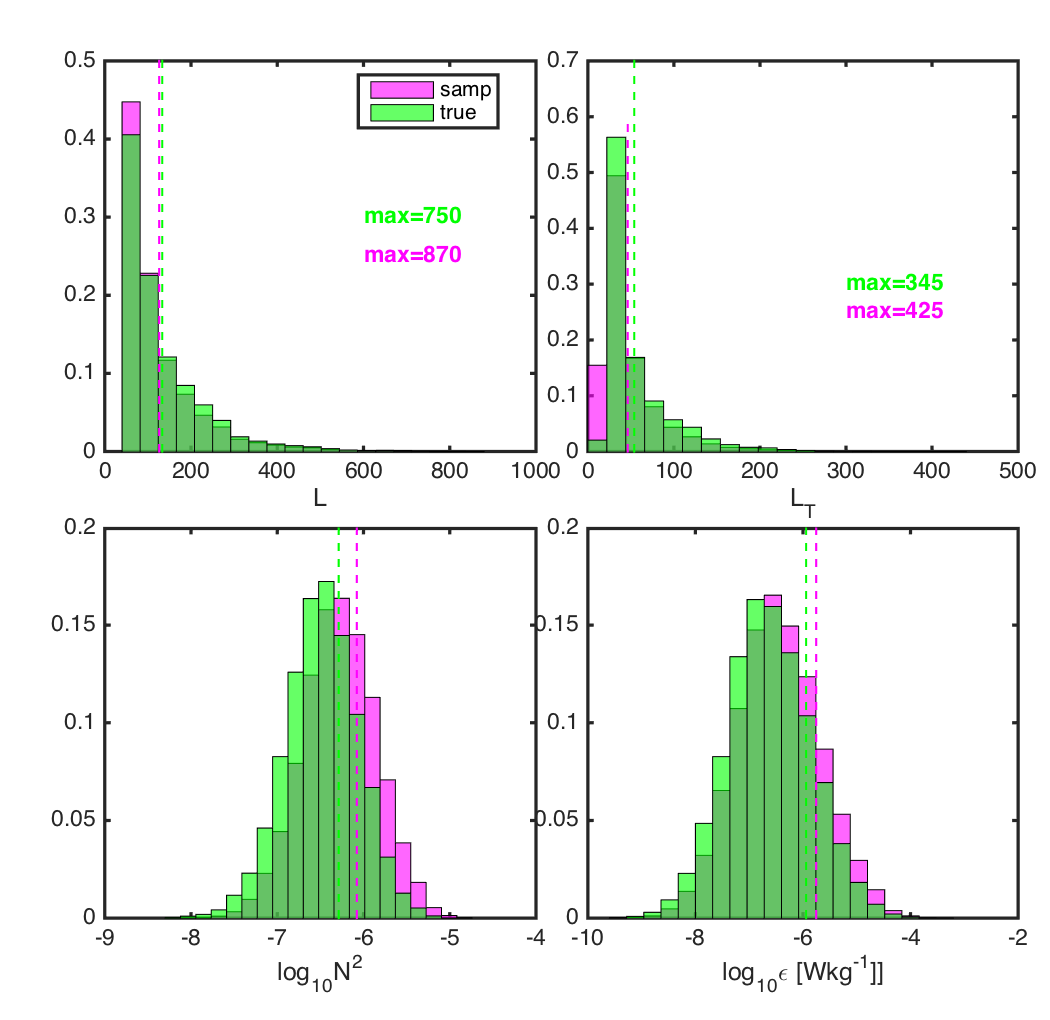
\includegraphics[width=38pc,angle=0]{../NotesOverturnBiases/Tchain3_2X2_Histograms.png}\\
  \caption{Histograms of epsilon for true and resampled data at T-chain 3. The mean of each distribution is indicated by the diamond and dashed line.}
  \label{hists}
\end{figure}



%~~~~~~~~~~~
\clearpage
%~~ CTD scenario
\begin{figure}[t]
  \noindent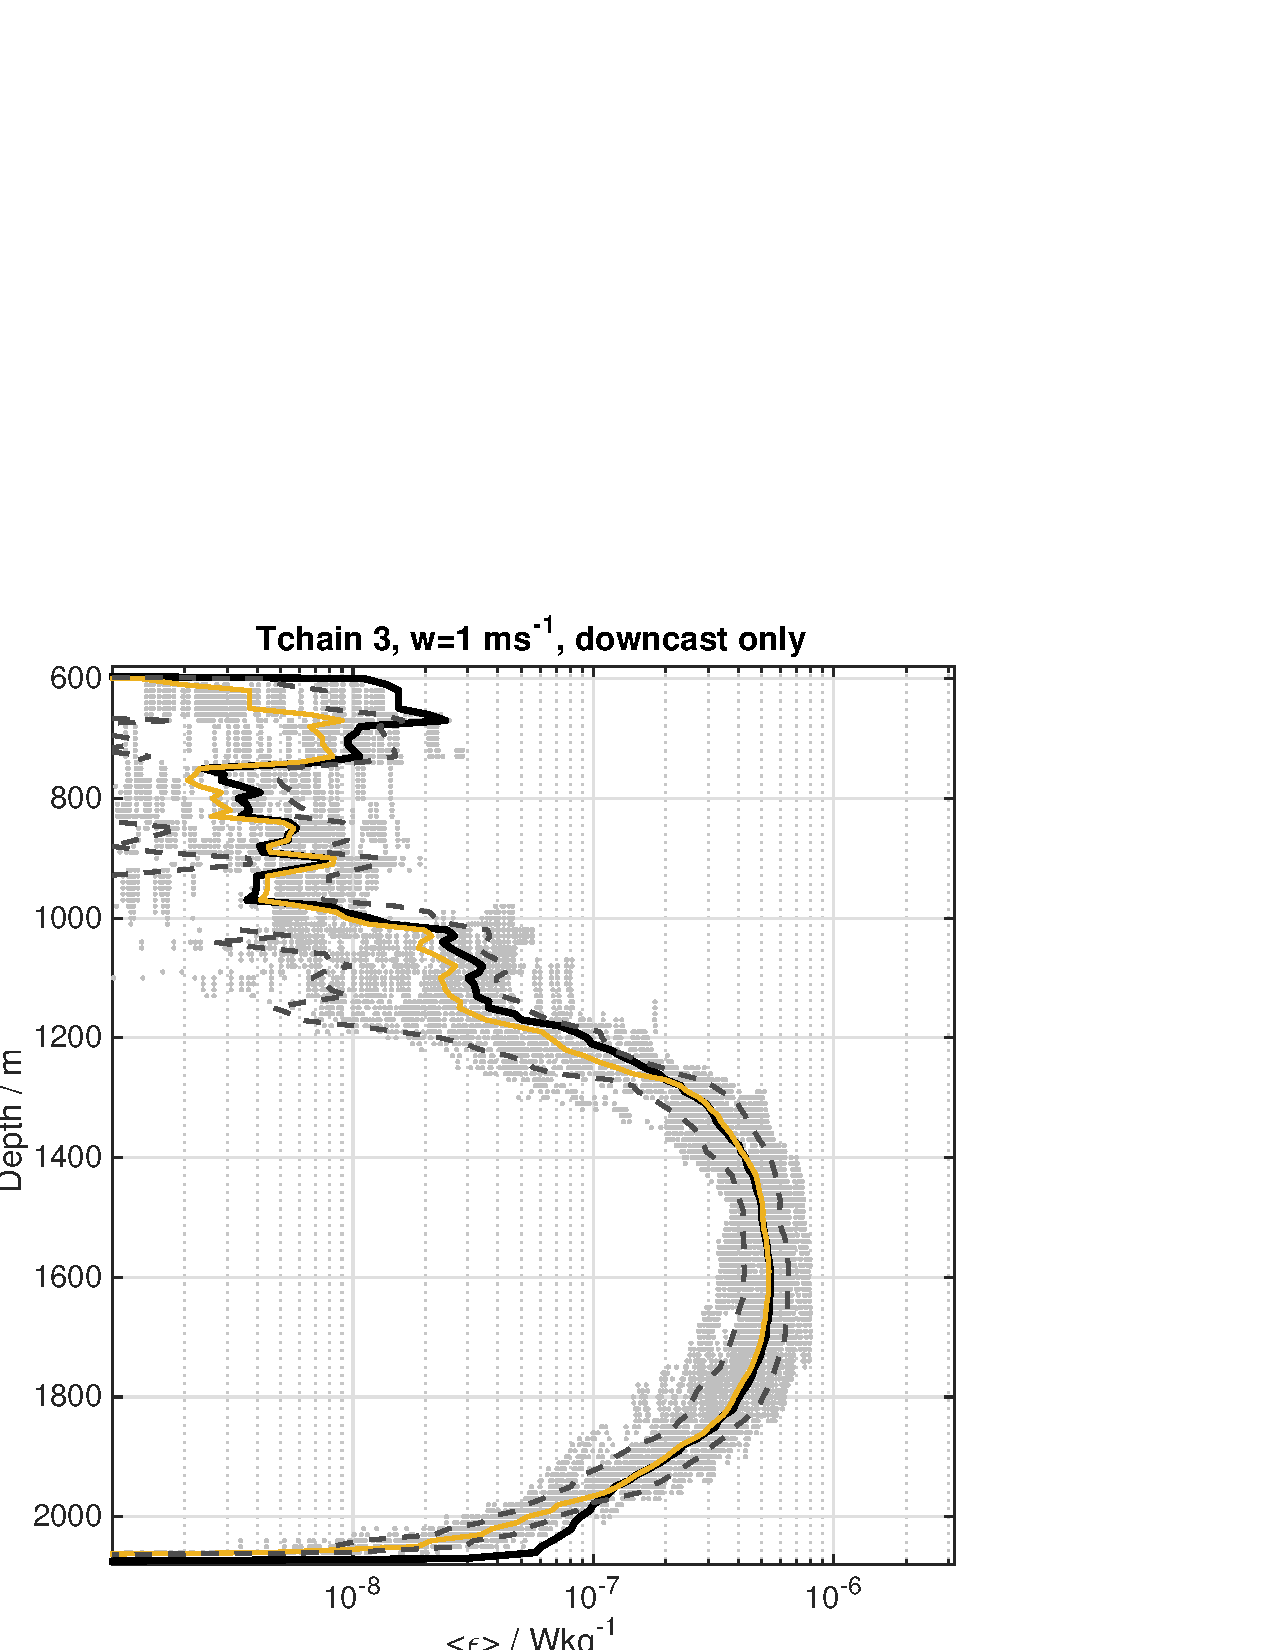
\includegraphics[width=38pc,angle=0]{../NotesOverturnBiases/Tchain3_Resamp_EpsvsDepth_CTDscenario.pdf}\\
  \caption{Profiles of time-mean epsilon for simulated sampling by a shipboard CTD profiling at $1\mathrm{ms^{-1}}$, using  downcasts only.}
  \label{T3_ctd_profile}
\end{figure}



%~~~~~~~~~~~
\clearpage
\begin{figure}[t]
  \noindent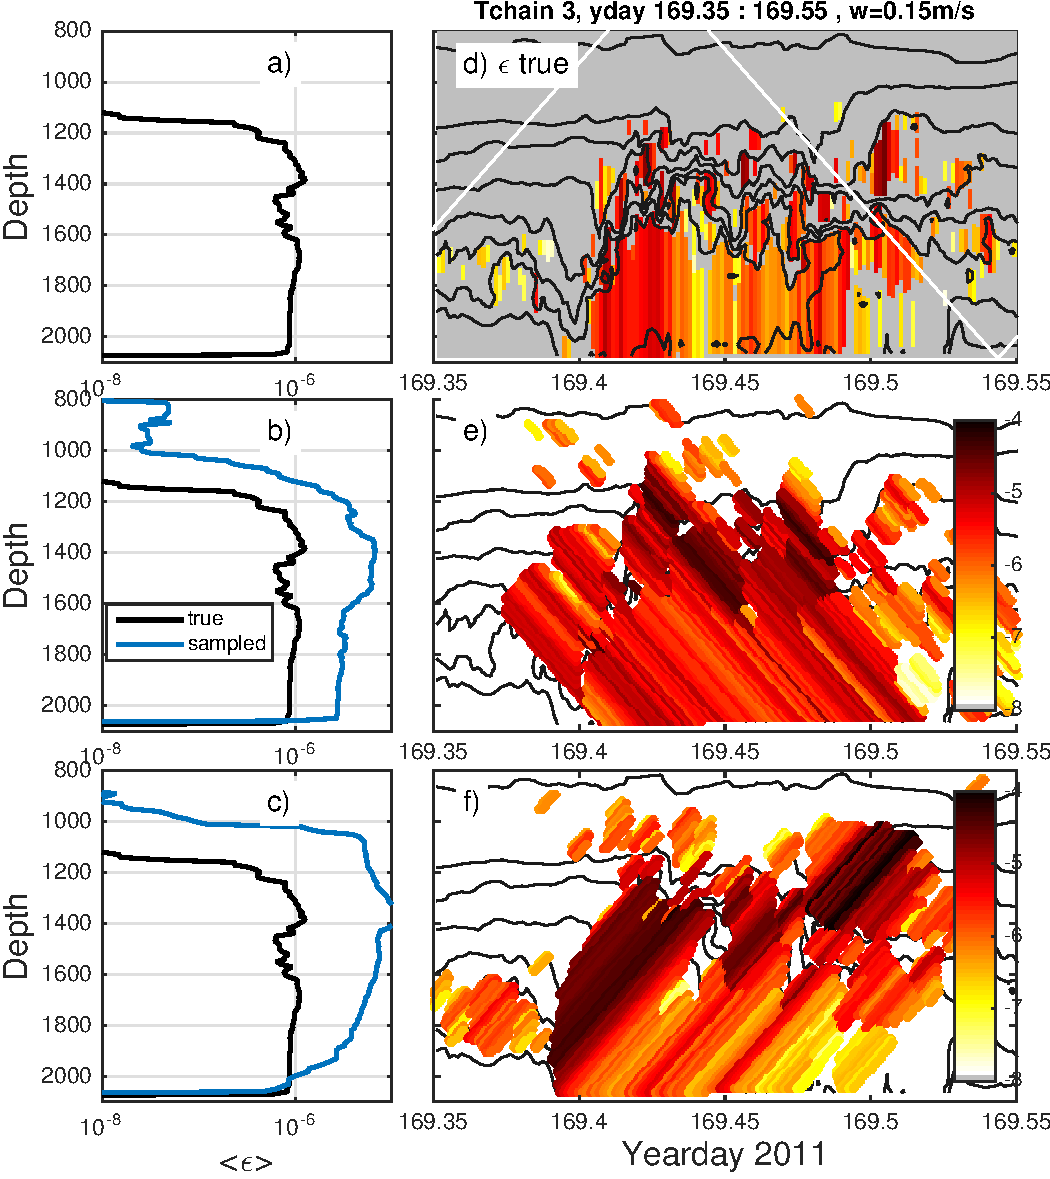
\includegraphics[width=38pc,angle=0]{../NotesOverturnBiases/Tchain3_AlongPath_NearDay169_Test_3.pdf}\\
  \caption{A detailed look at one turbulent period. (Top) Epsilon estimated from full T-chain data. (middle) Epsilon from overturns for downward sampling paths, plotted along each path in the ensemble. (bottom) Same as middle, but for upward paths. Colorscale for espilon is the same in all 3 panels. Left panels show time-average profile of true (black) and resampled (blue) $\epsilon$ for each case. Note the much larger epsilon where sampling paths are nearly parallel to slope of isopycnals.}
 \label{zoomex}
\end{figure}



%~~~~~~~~~~~
\clearpage
% histograms of difference in Lt
\begin{figure}[t]
  \noindent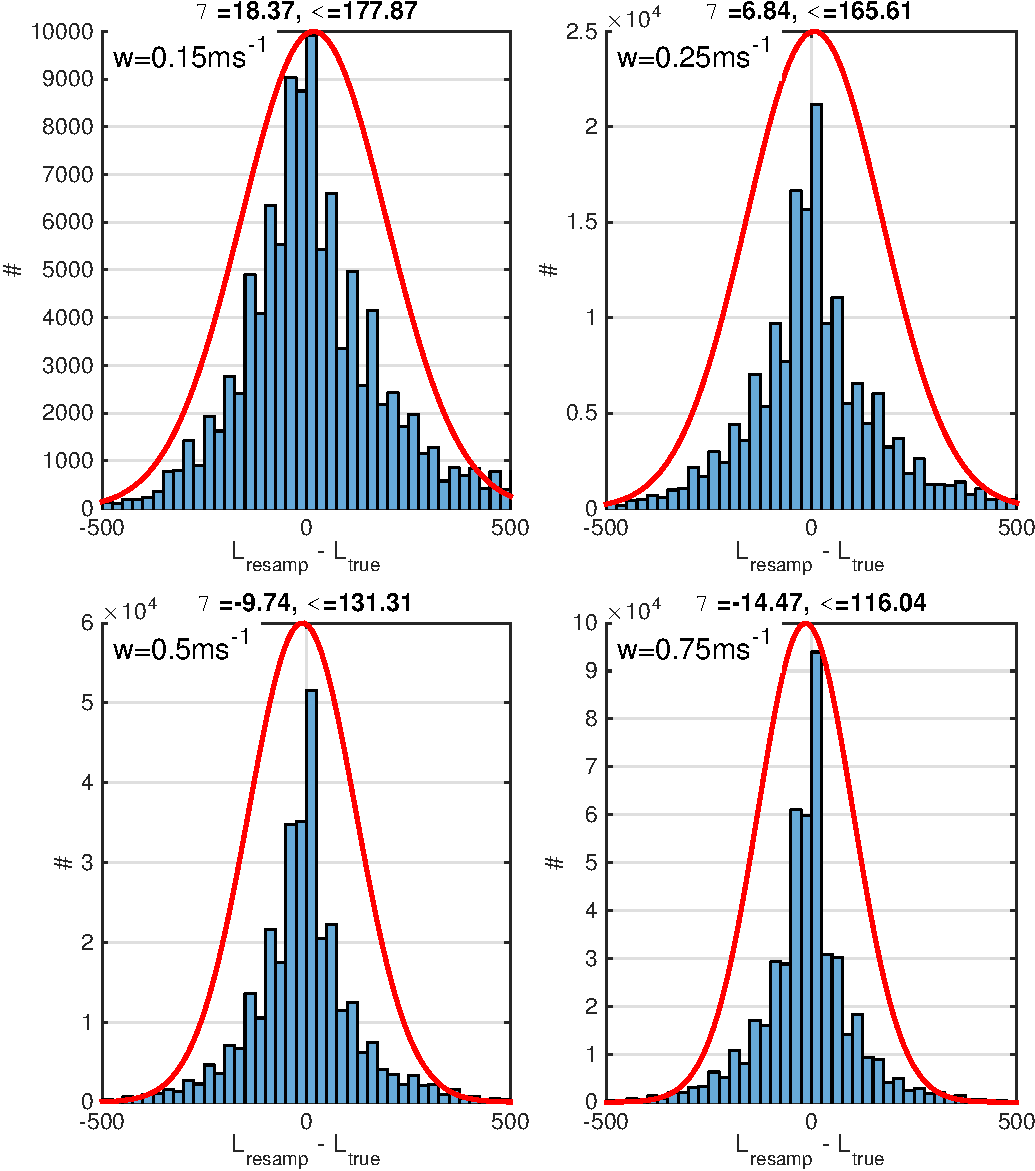
\includegraphics[width=38pc,angle=0]{../NotesOverturnBiases/Tchain3_LtDifHist_4Cases.pdf}\\
  \caption{Histograms of the difference between true and resampled overturn sizes for different profiling speeds at T-chain 3. The mean and standard deviation are given above each plot, and red lines show normal distributions with those parameters.}
  \label{T3LtDiffHists}
\end{figure}


%~~~~~~~~
\clearpage
% Correct_Resampled_Eps.m
\begin{figure}[t]
  \noindent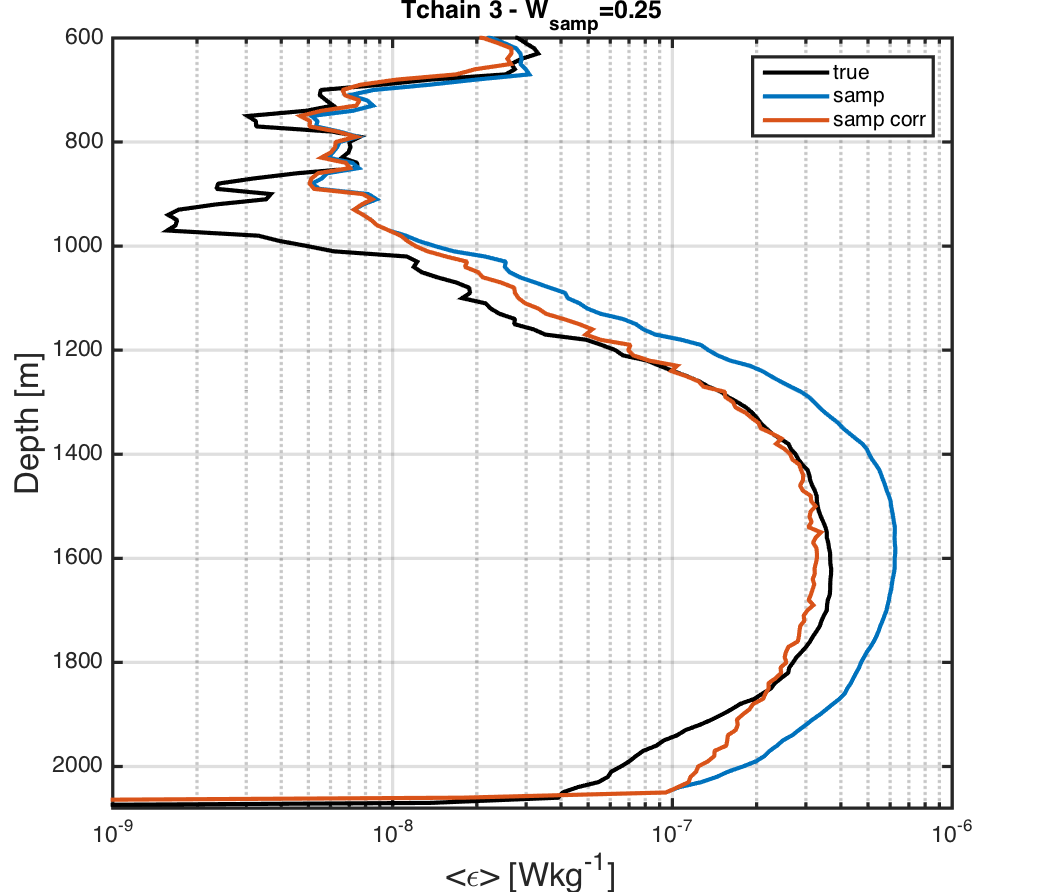
\includegraphics[width=38pc,angle=0]{../NotesOverturnBiases/Tchain3_Testnum1_Raw_corr_profiles.png}\\
  \caption{Time-average profiles of dissipation rate at T-chain 3. Black line is true value. Blue line is for resampled data with $w_{samp}=0.25$. Red line shows resampled data after discarding data where $w_t > 0.5 w_{samp}$ . }
  \label{T3_corrProf}
\end{figure}



\end{document}